% Options for packages loaded elsewhere
\PassOptionsToPackage{unicode}{hyperref}
\PassOptionsToPackage{hyphens}{url}
%
\documentclass[
]{article}
\usepackage{amsmath,amssymb}
\usepackage{iftex}
\ifPDFTeX
  \usepackage[T1]{fontenc}
  \usepackage[utf8]{inputenc}
  \usepackage{textcomp} % provide euro and other symbols
\else % if luatex or xetex
  \usepackage{unicode-math} % this also loads fontspec
  \defaultfontfeatures{Scale=MatchLowercase}
  \defaultfontfeatures[\rmfamily]{Ligatures=TeX,Scale=1}
\fi
\usepackage{lmodern}
\ifPDFTeX\else
  % xetex/luatex font selection
\fi
% Use upquote if available, for straight quotes in verbatim environments
\IfFileExists{upquote.sty}{\usepackage{upquote}}{}
\IfFileExists{microtype.sty}{% use microtype if available
  \usepackage[]{microtype}
  \UseMicrotypeSet[protrusion]{basicmath} % disable protrusion for tt fonts
}{}
\makeatletter
\@ifundefined{KOMAClassName}{% if non-KOMA class
  \IfFileExists{parskip.sty}{%
    \usepackage{parskip}
  }{% else
    \setlength{\parindent}{0pt}
    \setlength{\parskip}{6pt plus 2pt minus 1pt}}
}{% if KOMA class
  \KOMAoptions{parskip=half}}
\makeatother
\usepackage{xcolor}
\usepackage[margin=1in]{geometry}
\usepackage{color}
\usepackage{fancyvrb}
\newcommand{\VerbBar}{|}
\newcommand{\VERB}{\Verb[commandchars=\\\{\}]}
\DefineVerbatimEnvironment{Highlighting}{Verbatim}{commandchars=\\\{\}}
% Add ',fontsize=\small' for more characters per line
\usepackage{framed}
\definecolor{shadecolor}{RGB}{248,248,248}
\newenvironment{Shaded}{\begin{snugshade}}{\end{snugshade}}
\newcommand{\AlertTok}[1]{\textcolor[rgb]{0.94,0.16,0.16}{#1}}
\newcommand{\AnnotationTok}[1]{\textcolor[rgb]{0.56,0.35,0.01}{\textbf{\textit{#1}}}}
\newcommand{\AttributeTok}[1]{\textcolor[rgb]{0.13,0.29,0.53}{#1}}
\newcommand{\BaseNTok}[1]{\textcolor[rgb]{0.00,0.00,0.81}{#1}}
\newcommand{\BuiltInTok}[1]{#1}
\newcommand{\CharTok}[1]{\textcolor[rgb]{0.31,0.60,0.02}{#1}}
\newcommand{\CommentTok}[1]{\textcolor[rgb]{0.56,0.35,0.01}{\textit{#1}}}
\newcommand{\CommentVarTok}[1]{\textcolor[rgb]{0.56,0.35,0.01}{\textbf{\textit{#1}}}}
\newcommand{\ConstantTok}[1]{\textcolor[rgb]{0.56,0.35,0.01}{#1}}
\newcommand{\ControlFlowTok}[1]{\textcolor[rgb]{0.13,0.29,0.53}{\textbf{#1}}}
\newcommand{\DataTypeTok}[1]{\textcolor[rgb]{0.13,0.29,0.53}{#1}}
\newcommand{\DecValTok}[1]{\textcolor[rgb]{0.00,0.00,0.81}{#1}}
\newcommand{\DocumentationTok}[1]{\textcolor[rgb]{0.56,0.35,0.01}{\textbf{\textit{#1}}}}
\newcommand{\ErrorTok}[1]{\textcolor[rgb]{0.64,0.00,0.00}{\textbf{#1}}}
\newcommand{\ExtensionTok}[1]{#1}
\newcommand{\FloatTok}[1]{\textcolor[rgb]{0.00,0.00,0.81}{#1}}
\newcommand{\FunctionTok}[1]{\textcolor[rgb]{0.13,0.29,0.53}{\textbf{#1}}}
\newcommand{\ImportTok}[1]{#1}
\newcommand{\InformationTok}[1]{\textcolor[rgb]{0.56,0.35,0.01}{\textbf{\textit{#1}}}}
\newcommand{\KeywordTok}[1]{\textcolor[rgb]{0.13,0.29,0.53}{\textbf{#1}}}
\newcommand{\NormalTok}[1]{#1}
\newcommand{\OperatorTok}[1]{\textcolor[rgb]{0.81,0.36,0.00}{\textbf{#1}}}
\newcommand{\OtherTok}[1]{\textcolor[rgb]{0.56,0.35,0.01}{#1}}
\newcommand{\PreprocessorTok}[1]{\textcolor[rgb]{0.56,0.35,0.01}{\textit{#1}}}
\newcommand{\RegionMarkerTok}[1]{#1}
\newcommand{\SpecialCharTok}[1]{\textcolor[rgb]{0.81,0.36,0.00}{\textbf{#1}}}
\newcommand{\SpecialStringTok}[1]{\textcolor[rgb]{0.31,0.60,0.02}{#1}}
\newcommand{\StringTok}[1]{\textcolor[rgb]{0.31,0.60,0.02}{#1}}
\newcommand{\VariableTok}[1]{\textcolor[rgb]{0.00,0.00,0.00}{#1}}
\newcommand{\VerbatimStringTok}[1]{\textcolor[rgb]{0.31,0.60,0.02}{#1}}
\newcommand{\WarningTok}[1]{\textcolor[rgb]{0.56,0.35,0.01}{\textbf{\textit{#1}}}}
\usepackage{longtable,booktabs,array}
\usepackage{calc} % for calculating minipage widths
% Correct order of tables after \paragraph or \subparagraph
\usepackage{etoolbox}
\makeatletter
\patchcmd\longtable{\par}{\if@noskipsec\mbox{}\fi\par}{}{}
\makeatother
% Allow footnotes in longtable head/foot
\IfFileExists{footnotehyper.sty}{\usepackage{footnotehyper}}{\usepackage{footnote}}
\makesavenoteenv{longtable}
\usepackage{graphicx}
\makeatletter
\def\maxwidth{\ifdim\Gin@nat@width>\linewidth\linewidth\else\Gin@nat@width\fi}
\def\maxheight{\ifdim\Gin@nat@height>\textheight\textheight\else\Gin@nat@height\fi}
\makeatother
% Scale images if necessary, so that they will not overflow the page
% margins by default, and it is still possible to overwrite the defaults
% using explicit options in \includegraphics[width, height, ...]{}
\setkeys{Gin}{width=\maxwidth,height=\maxheight,keepaspectratio}
% Set default figure placement to htbp
\makeatletter
\def\fps@figure{htbp}
\makeatother
\setlength{\emergencystretch}{3em} % prevent overfull lines
\providecommand{\tightlist}{%
  \setlength{\itemsep}{0pt}\setlength{\parskip}{0pt}}
\setcounter{secnumdepth}{-\maxdimen} % remove section numbering
\ifLuaTeX
  \usepackage{selnolig}  % disable illegal ligatures
\fi
\usepackage{bookmark}
\IfFileExists{xurl.sty}{\usepackage{xurl}}{} % add URL line breaks if available
\urlstyle{same}
\hypersetup{
  pdftitle={Supplementary Information: Older participants are slower in a visual lexical decision task, but this is attenuated by a large vocabulary},
  pdfauthor={Rácz, Péter},
  hidelinks,
  pdfcreator={LaTeX via pandoc}}

\title{Supplementary Information: Older participants are slower in a
visual lexical decision task, but this is attenuated by a large
vocabulary}
\author{Rácz, Péter}
\date{2 October, 2024}

\begin{document}
\maketitle

\subsection{Links}\label{links}

The code to run the experiments on Gitlab for pilot 1, pilot 2, and the
main experiment are
\href{https://gitlab.pavlovia.org/petyaraczbme/lex_span4}{\textbf{here}},
\href{https://gitlab.pavlovia.org/petyaraczbme/lendulet_bme_szokiserlet_vegso}{\textbf{here}},
and
\href{https://gitlab.pavlovia.org/petyaraczbme/lex-dec-task-random}{\textbf{here}}.

\subsection{File structure and
workflow}\label{file-structure-and-workflow}

We ran two pilot experiments and a main experiment. The stimulus list
for pilot 1 was based on a frequency list from
\href{https://hlt.bme.hu/en/resources/webcorpus2}{Hungarian Webcorpus
2}. We host this list in this repository. Cite us and the original if
you want to use it. Subsequent stimulus lists were based on results from
pilot 1.

\begin{itemize}
\tightlist
\item
  src: corpus data in various processed forms
\item
  raw: raw output of the Gitlab scripts running the experiments
\item
  scripts: scripts to create the word lists, process the raw data,
  create the tidy data, and check on the processing
\item
  tidy: tidy data for pilot 1, 2, and main
\item
  analysis: scripts to analyse the tidy data from the main experiment
\end{itemize}

\subsection{Data dictionary for main data
(tidy/d.tsv)}\label{data-dictionary-for-main-data-tidyd.tsv}

\begin{itemize}
\tightlist
\item
  id\_spec: participant id with timestamp
\item
  n\_mistakes\_for\_nonce\_words: n times participant said yes to
  non-word
\item
  percent\_mistakes\_for\_nonce\_words: \% participant said yes to
  non-word
\item
  id: participant id
\item
  data\_type: did participant finish exp (they all did)
\item
  participant\_cap\_2: counting participant vocab size v2
\item
  participant\_cap\_1: counting participant vocab size v1
\item
  max\_trial\_number: 250 for everyone
\item
  max\_block: 50 for everyone
\item
  n\_mistakes\_for\_real\_words\_total
\item
  block
\item
  n\_mistakes\_for\_real\_words\_per\_bin:n times part said no to real
  word
\item
  yob: year of birth
\item
  edu: years spent in education
\item
  start: starting experiment
\item
  exp: this is exp3
\item
  row\_number: row number in data
\item
  block\_trial\_number: trial n 1-250 (only one block)
\item
  trial\_number: trial n 1-250
\item
  word: target
\item
  resp.keys: what key did part press
\item
  resp.rt: part time \textless- this is the outcome variable
\item
  pos: target part of speech
\item
  bin: target familiarity bin
\item
  lfpm10r: log freq per 10 mil in Webcorpus 2, scaled
\item
  nonce\_word: this is a non-word
\item
  correct: correct answer (y for word, n for non-word)
\item
  link: link to exp
\item
  missed\_nonce\_words: n non-words missed by part
\item
  gender: part gender, self reported
\item
  drop\_participant: part meets exclusion criteria
\item
  drop\_observation: response meets exclusion criteria
\item
  year\_of\_birth: year of birth tidy
\item
  start\_time: start time tidy
\item
  start\_year: start year
\item
  age: year - yob
\item
  answer: yes or no
\item
  participant\_age: age \textless- predictor
\item
  participant\_vocabulary\_size: vocab size \textless- predictor
\item
  word\_familiarity: word familiarity bin \textless- predictor
\end{itemize}

\subsection{Exclusion criteria}\label{exclusion-criteria}

\begin{itemize}
\tightlist
\item
  drop\_participant = missed\_nonce\_words \textgreater{} 20
\item
  drop\_observation = resp.rt \textgreater{} 4
\end{itemize}

\begin{Shaded}
\begin{Highlighting}[]
\CommentTok{\# n obs}
\FunctionTok{nrow}\NormalTok{(d)}
\end{Highlighting}
\end{Shaded}

\begin{verbatim}
## [1] 71608
\end{verbatim}

\begin{Shaded}
\begin{Highlighting}[]
\CommentTok{\# n part}
\FunctionTok{length}\NormalTok{(}\FunctionTok{unique}\NormalTok{(d}\SpecialCharTok{$}\NormalTok{id\_spec))}
\end{Highlighting}
\end{Shaded}

\begin{verbatim}
## [1] 467
\end{verbatim}

\begin{Shaded}
\begin{Highlighting}[]
\CommentTok{\# n filt obs}
\FunctionTok{nrow}\NormalTok{(filt)}
\end{Highlighting}
\end{Shaded}

\begin{verbatim}
## [1] 113076
\end{verbatim}

\begin{Shaded}
\begin{Highlighting}[]
\CommentTok{\# n filt part}
\FunctionTok{length}\NormalTok{(}\FunctionTok{unique}\NormalTok{(filt}\SpecialCharTok{$}\NormalTok{id\_spec))}
\end{Highlighting}
\end{Shaded}

\begin{verbatim}
## [1] 472
\end{verbatim}

\begin{Shaded}
\begin{Highlighting}[]
\CommentTok{\# filt counts}
\NormalTok{filt }\SpecialCharTok{|\textgreater{}} 
  \FunctionTok{count}\NormalTok{(nonce\_word,correct) }\SpecialCharTok{|\textgreater{}} 
  \FunctionTok{pivot\_wider}\NormalTok{(}\AttributeTok{names\_from =}\NormalTok{ nonce\_word, }\AttributeTok{values\_from =}\NormalTok{ n) }\SpecialCharTok{|\textgreater{}} 
  \FunctionTok{rename}\NormalTok{(}\StringTok{\textquotesingle{}non word\textquotesingle{}} \OtherTok{=} \StringTok{\textasciigrave{}}\AttributeTok{TRUE}\StringTok{\textasciigrave{}}\NormalTok{, }\StringTok{\textquotesingle{}real word\textquotesingle{}} \OtherTok{=} \StringTok{\textasciigrave{}}\AttributeTok{FALSE}\StringTok{\textasciigrave{}}\NormalTok{) }\SpecialCharTok{|\textgreater{}} 
  \FunctionTok{mutate}\NormalTok{(}\AttributeTok{response =} \FunctionTok{ifelse}\NormalTok{(correct, }\StringTok{\textquotesingle{}yes\textquotesingle{}}\NormalTok{, }\StringTok{\textquotesingle{}no\textquotesingle{}}\NormalTok{)) }\SpecialCharTok{|\textgreater{}} 
  \FunctionTok{select}\NormalTok{(response,}\StringTok{\textasciigrave{}}\AttributeTok{real word}\StringTok{\textasciigrave{}}\NormalTok{,}\StringTok{\textasciigrave{}}\AttributeTok{non word}\StringTok{\textasciigrave{}}\NormalTok{) }\SpecialCharTok{|\textgreater{}} 
  \FunctionTok{kable}\NormalTok{(}\StringTok{\textquotesingle{}simple\textquotesingle{}}\NormalTok{)}
\end{Highlighting}
\end{Shaded}

\begin{longtable}[]{@{}lrr@{}}
\toprule\noalign{}
response & real word & non word \\
\midrule\noalign{}
\endhead
\bottomrule\noalign{}
\endlastfoot
no & 18016 & 1977 \\
yes & 72365 & 20718 \\
\end{longtable}

\begin{Shaded}
\begin{Highlighting}[]
\CommentTok{\# young}
\FunctionTok{nrow}\NormalTok{(idsy)}
\end{Highlighting}
\end{Shaded}

\begin{verbatim}
## [1] 80
\end{verbatim}

\begin{Shaded}
\begin{Highlighting}[]
\CommentTok{\# old}
\FunctionTok{nrow}\NormalTok{(idso)}
\end{Highlighting}
\end{Shaded}

\begin{verbatim}
## [1] 387
\end{verbatim}

\subsection{Model comparison}\label{model-comparison}

Three models fit on young and old data. lme4. ML. for main and resid
models, participant and word random intercept plus word familiarity
slope for participant. AIC, BIC, likelihood ratio test used for model
comparison. Models checked for collinearity using variance inflation
factor. (age and vocab size very collinear, so we decided not to test
interactions directly).

Young data: - Vocabulary: Is the vocabulary x age relationship linear or
polynomial? - Main: RT \textasciitilde{} part age, vocab size, word
familiarity - Resid Vocab/Age: RT \textasciitilde{} part age, variation
in vocab size not explained by age (residualised vocabulary size), word
familiarity

\begin{Shaded}
\begin{Highlighting}[]
\CommentTok{\# best models:}

\DocumentationTok{\#\# {-}{-} young {-}{-} \#\#}

\DocumentationTok{\#\# vocabulary}
\NormalTok{myv1 }\OtherTok{=} \FunctionTok{lm}\NormalTok{(s\_size }\SpecialCharTok{\textasciitilde{}}\NormalTok{ s\_age, }\AttributeTok{data =}\NormalTok{ idsy)}
\DocumentationTok{\#\# main}
\NormalTok{mys1 }\OtherTok{=} \FunctionTok{lmer}\NormalTok{(resp.rt }\SpecialCharTok{\textasciitilde{}} \DecValTok{1} \SpecialCharTok{+}\NormalTok{ s\_age }\SpecialCharTok{+}\NormalTok{ s\_word }\SpecialCharTok{+}\NormalTok{ s\_size }\SpecialCharTok{+}\NormalTok{ (}\DecValTok{1}\SpecialCharTok{+}\NormalTok{s\_word}\SpecialCharTok{|}\NormalTok{id) }\SpecialCharTok{+}\NormalTok{ (}\DecValTok{1}\SpecialCharTok{|}\NormalTok{word), }\AttributeTok{data =}\NormalTok{ young, }\AttributeTok{REML =}\NormalTok{ F, }\AttributeTok{control =} \FunctionTok{lmerControl}\NormalTok{(}\AttributeTok{optimizer=}\StringTok{"bobyqa"}\NormalTok{, }\AttributeTok{optCtrl=}\FunctionTok{list}\NormalTok{(}\AttributeTok{maxfun=}\DecValTok{20000}\NormalTok{)))}
\DocumentationTok{\#\# residualised}
\NormalTok{myr1 }\OtherTok{=} \FunctionTok{lmer}\NormalTok{(resp.rt }\SpecialCharTok{\textasciitilde{}} \DecValTok{1} \SpecialCharTok{+}\NormalTok{ s\_age }\SpecialCharTok{+}\NormalTok{ res\_size\_age }\SpecialCharTok{+}\NormalTok{ s\_word }\SpecialCharTok{+}\NormalTok{ (}\DecValTok{1}\SpecialCharTok{+}\NormalTok{s\_word}\SpecialCharTok{|}\NormalTok{id) }\SpecialCharTok{+}\NormalTok{ (}\DecValTok{1}\SpecialCharTok{|}\NormalTok{word), }\AttributeTok{data =}\NormalTok{ young, }\AttributeTok{REML =}\NormalTok{ F, }\AttributeTok{control =} \FunctionTok{lmerControl}\NormalTok{(}\AttributeTok{optimizer=}\StringTok{"bobyqa"}\NormalTok{, }\AttributeTok{optCtrl=}\FunctionTok{list}\NormalTok{(}\AttributeTok{maxfun=}\DecValTok{20000}\NormalTok{)))}
\end{Highlighting}
\end{Shaded}

Young data: - Vocabulary: Is the vocabulary x age relationship linear or
polynomial? - Main: RT \textasciitilde{} part age, vocab size,
education, word familiarity - Resid Vocab/Age: RT \textasciitilde{} part
edu, age, variation in vocab size not explained by age (residualised
vocabulary size), word familiarity - Resid Vocab/Edu: RT
\textasciitilde{} part age, edu, variation in vocab size not explained
by edu (residualised vocabulary size), word familiarity

\begin{Shaded}
\begin{Highlighting}[]
\CommentTok{\# best models ctd.:}

\DocumentationTok{\#\# {-}{-} old {-}{-} \#\#}

\DocumentationTok{\#\# vocabulary}
\NormalTok{mov1 }\OtherTok{=} \FunctionTok{lm}\NormalTok{(s\_size }\SpecialCharTok{\textasciitilde{}} \DecValTok{1} \SpecialCharTok{+}\NormalTok{ s\_edu }\SpecialCharTok{+}\NormalTok{ s\_age, }\AttributeTok{data =}\NormalTok{ idso)}
\DocumentationTok{\#\# main}
\NormalTok{mos1 }\OtherTok{=} \FunctionTok{lmer}\NormalTok{(resp.rt }\SpecialCharTok{\textasciitilde{}} \DecValTok{1} \SpecialCharTok{+}\NormalTok{ s\_age }\SpecialCharTok{+}\NormalTok{ s\_edu }\SpecialCharTok{+}\NormalTok{ s\_word }\SpecialCharTok{+}\NormalTok{ s\_size }\SpecialCharTok{+}\NormalTok{ (}\DecValTok{1}\SpecialCharTok{+}\NormalTok{s\_word}\SpecialCharTok{|}\NormalTok{id) }\SpecialCharTok{+}\NormalTok{ (}\DecValTok{1}\SpecialCharTok{|}\NormalTok{word), }\AttributeTok{data =}\NormalTok{ old, }\AttributeTok{REML =}\NormalTok{ F, }\AttributeTok{control =} \FunctionTok{lmerControl}\NormalTok{(}\AttributeTok{optimizer=}\StringTok{"bobyqa"}\NormalTok{, }\AttributeTok{optCtrl=}\FunctionTok{list}\NormalTok{(}\AttributeTok{maxfun=}\DecValTok{20000}\NormalTok{)))}
\DocumentationTok{\#\# residualised}
\NormalTok{mor3 }\OtherTok{=} \FunctionTok{lmer}\NormalTok{(resp.rt }\SpecialCharTok{\textasciitilde{}} \DecValTok{1} \SpecialCharTok{+}\NormalTok{ s\_edu }\SpecialCharTok{+}\NormalTok{ s\_word }\SpecialCharTok{+}\NormalTok{ res\_size\_age }\SpecialCharTok{*}\NormalTok{ s\_age }\SpecialCharTok{+}\NormalTok{ (}\DecValTok{1}\SpecialCharTok{+}\NormalTok{s\_word}\SpecialCharTok{|}\NormalTok{id) }\SpecialCharTok{+}\NormalTok{ (}\DecValTok{1}\SpecialCharTok{|}\NormalTok{word), }\AttributeTok{data =}\NormalTok{ old, }\AttributeTok{REML =}\NormalTok{ F, }\AttributeTok{control =} \FunctionTok{lmerControl}\NormalTok{(}\AttributeTok{optimizer=}\StringTok{"bobyqa"}\NormalTok{, }\AttributeTok{optCtrl=}\FunctionTok{list}\NormalTok{(}\AttributeTok{maxfun=}\DecValTok{20000}\NormalTok{)))}
\NormalTok{mor4 }\OtherTok{=} \FunctionTok{lmer}\NormalTok{(resp.rt }\SpecialCharTok{\textasciitilde{}} \DecValTok{1} \SpecialCharTok{+}\NormalTok{ s\_age }\SpecialCharTok{+}\NormalTok{ s\_word }\SpecialCharTok{+}\NormalTok{ res\_size\_edu }\SpecialCharTok{*}\NormalTok{ s\_edu }\SpecialCharTok{+}\NormalTok{ (}\DecValTok{1}\SpecialCharTok{+}\NormalTok{s\_word}\SpecialCharTok{|}\NormalTok{id) }\SpecialCharTok{+}\NormalTok{ (}\DecValTok{1}\SpecialCharTok{|}\NormalTok{word), }\AttributeTok{data =}\NormalTok{ old, }\AttributeTok{REML =}\NormalTok{ F, }\AttributeTok{control =} \FunctionTok{lmerControl}\NormalTok{(}\AttributeTok{optimizer=}\StringTok{"bobyqa"}\NormalTok{, }\AttributeTok{optCtrl=}\FunctionTok{list}\NormalTok{(}\AttributeTok{maxfun=}\DecValTok{20000}\NormalTok{)))}
\end{Highlighting}
\end{Shaded}

\subsection{Plots in paper}\label{plots-in-paper}

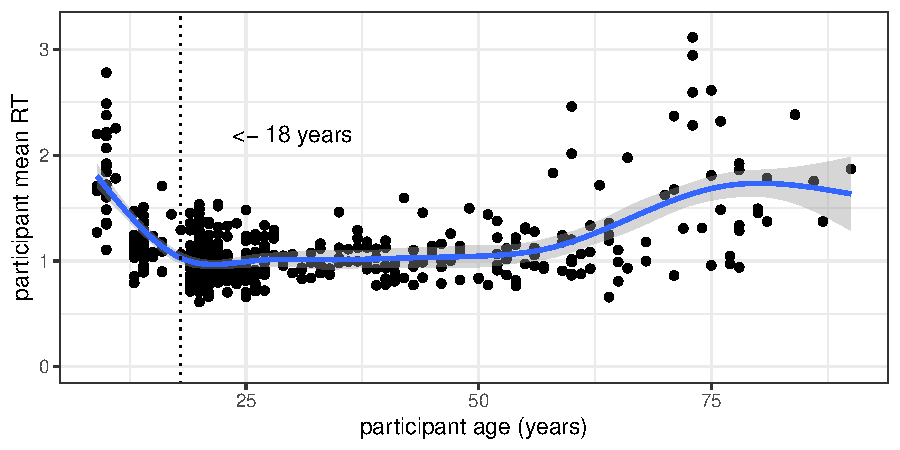
\includegraphics{figures/plot1-1.pdf}

\end{document}
